\documentclass[12pt]{article}
%Gummi|065|=)
\usepackage{amsmath, amsfonts, amssymb}
\usepackage[margin=0.5in]{geometry}
\usepackage{xcolor}
%\usepackage{graphicx}
%\usepackage{graphicx}
\newcommand{\off}[1]{}
\DeclareMathSizes{20}{30}{21}{18}

\newcommand{\myhrule}{}

\usepackage{tikz}

\title{\textbf{ Examples:  Theta Functions}}
\author{John D Mangual}
\date{}
\begin{document}

\fontfamily{qag}\selectfont \fontsize{25}{30}\selectfont

\maketitle

\noindent  Conformal field theory is a central topic in mathematical physics\footnote{What does that even mean?  Here it means there are other math problems  in fields like Number Theory and Topology and Chern Simons Theory -- and specific sources -- which point to the paper we will review today. }.  What is Conformal Field Theory? \\
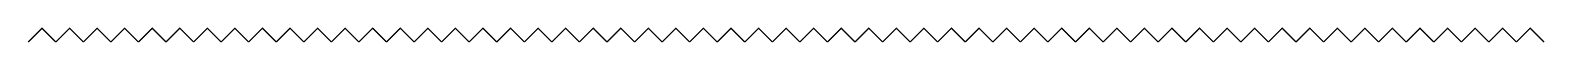
\begin{tikzpicture}[scale=0.35]
\foreach \x in {1,...,55}{
	\draw (\x,-0.25)--(\x+0.5,0.25)--(\x+1,-0.25);
}
\end{tikzpicture}
The rational gaussian model has a single scalar free field $\phi$ which is compactified on a circle with $R^2 \in \mathbb{Q}$.  \\ \\
This theory has a large group of symmetries -- an extension of the the $U(1)$ current algebra. \\ \\
The $N$ primary fields $[\phi_p]$ are vertex-operators with momentum $\frac{p}{\sqrt{N}}$ and $p \in \mathbb{Z}_N$. \\ \\
The fusion rules are $\phi_p \times \phi_q = \phi_{p+q}$ with $p,q \in \mathbb{Z}$.

\newpage

\noindent The discussion the last page is already quite problematic.  Why is $R^2 \in \mathbb{Q}$ , e.g. $R = \sqrt{3}$? \\ \\
It seems I have confused $\phi$ and $\varphi$.  These are related by the exponential function:
$$ \phi_p ( \textbf{c} )
= \exp \left( \frac{p}{\sqrt{N}} 
\int_\textbf{c} \partial \varphi \right)$$
this is such a nice looking integrals with nice properties:
$$ 
\phi_p ( \textbf{a} )
\phi_q ( \textbf{b} )
= 
e^{ 2\pi i \, pq/N}
\phi_q ( \textbf{b} )
\phi_p ( \textbf{a} )
$$
Now I want to know why these feel like the basic commutation operators from Quantum Mechanics:
$$ [x, p] = -i \hbar $$
and you can even prove these yourself, right? Let $p = -i\hbar \frac{d}{dx}$ then:
$$ \left[ x, i\hbar \frac{d}{dx} \right]f(x)
= i\hbar \left( x \frac{df}{dx}  - 
x\frac{df}{dx} + \frac{dx}{dx}f\right) = -i\hbar $$
Expect we are getting the exponentiated form.  That's it\footnote{I am not going to review anything more from Verlinde's paper -- I will be too busy making sense of these objects to discuss anything else.}

\newpage

\noindent Excuse me, Verline talks about the $S$ and $T$ operators.  The first one is clear:
$$ S: \chi_p \to \frac{1}{\sqrt{N}} \sum_{q \in \mathbb{Z}_N} e^{2\pi i \, pq / N}\chi_q $$
The only $\textit{S}$ and $\textit{T}$ operators that I know very well act on a Torus:
$$ S: 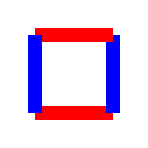
\begin{tikzpicture}
\draw[color= red, line width=5pt] (0,0)--(1,0);
\draw[color=blue, line width=5pt] (1,0)--(1,1);
\draw[color= red, line width=5pt] (1,1)--(0,1);
\draw[color=blue, line width=5pt] (0,1)--(0,0);
\end{tikzpicture} \to 
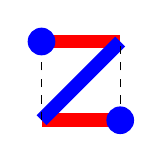
\begin{tikzpicture}
\draw[color= red, line width=5pt] (0,0)--(1,0);
\draw[color=blue, line width=5pt] (0,1) circle (1pt);
\draw[color= red, line width=5pt] (1,1)--(0,1);
\draw[color=blue, line width=5pt] (1,1)--(0,0);

\draw[dashed] (0,0)--(0,1);
\draw[dashed] (1,0)--(1,1);

\fill[color=blue] (0,1) circle (5pt);
\fill[color=blue] (1,0) circle (5pt);
\end{tikzpicture}
 $$
The other operator flips the torus (a technical term):
$$ T: 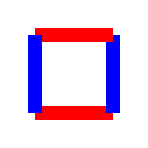
\begin{tikzpicture}
\draw[color= red, line width=5pt] (0,0)--(1,0);
\draw[color=blue, line width=5pt] (1,0)--(1,1);
\draw[color= red, line width=5pt] (1,1)--(0,1);
\draw[color=blue, line width=5pt] (0,1)--(0,0);
\end{tikzpicture} \to 
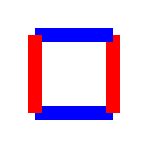
\begin{tikzpicture}
\draw[color=blue, line width=5pt] (0,0)--(1,0);
\draw[color= red, line width=5pt] (1,0)--(1,1);
\draw[color=blue, line width=5pt] (1,1)--(0,1);
\draw[color= red, line width=5pt] (0,1)--(0,0);
\end{tikzpicture}
 $$
This action lifts to \textbf{observable} that happens on that torus.  
$$ T: \chi_p \to e^{2\pi i \, p /N}\chi_p $$
With some effort these can happen on an octagon\footnote{Perhaps I should draw these by hand first!}\\
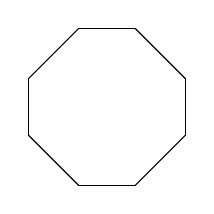
\begin{tikzpicture}
\draw (1, -0.356)--(1  , 0.356);
\draw (1,  0.356)--(0.356,   1);
\draw (0.356, 1) -- (-0.356, 1);
\draw (-0.356, 1)--(-1, 0.356);
\draw (-1, 0.356)--(-1,-0.356);
\draw (-1, -0.356)--(-0.356,-1);
\draw (-0.356, -1)--(0.356, -1);
\draw (0.356, -1)--(1, -0.356);
\end{tikzpicture}
...
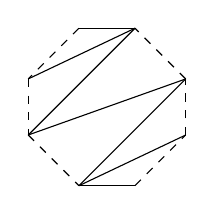
\begin{tikzpicture}
\draw[dashed] (1, -0.356)--(1  , 0.356);
\draw[dashed] (1,  0.356)--(0.356,   1);
\draw (0.356, 1) -- (-0.356, 1);
\draw[dashed] (-0.356, 1)--(-1, 0.356);
\draw (-1, 0.356)--(0.356,1);
\draw[dashed] (-1, 0.356)--(-1,-0.356);
\draw (-1, -0.356)--(1, 0.356);
\draw[dashed] (-1, -0.356)--(-0.356,-1);
\draw (-0.356, -1)--(0.356, -1);
\draw (-0.356, -1)--(1, -0.356);
\draw[dashed] (0.356, -1)--(1, -0.356);
\draw (-1, -0.356)--(0.356, 1);
\draw (-0.356,-1)--(1, 0.356);
\end{tikzpicture} \\
Verlinde's big result is: \textbf{the modular transformation $S$ diagonalizes the fusion rules}\footnote{See?  We can recite these formulas over and over many times with no idea what they mean :-)}
$$ \phi_p \times \phi_q = \phi_{p+q} $$



\newpage

\fontfamily{qag}\selectfont \fontsize{12}{10}\selectfont


\begin{thebibliography}{}

\item Erik Verlinde. \textbf{Fusion rules and modular transformations in 2D conformal field theory.} \\ Nuclear Physics B
Volume 300, 1988, Pages 360-376


\end{thebibliography}



\end{document}